%% JSAMS Brief Report — supplementary material (anonymised). Tables S1–S5 as in the full
%% submission; S6 and Figures S1–S3 are the display items moved out of the main text.
\documentclass[12pt,a4paper]{article}
\usepackage[utf8]{inputenc}
\usepackage[T1]{fontenc}
\usepackage{times}
\usepackage[margin=2.5cm]{geometry}
\usepackage{float}
\usepackage{booktabs}
\usepackage{caption}
\usepackage{graphicx}
\graphicspath{{../figures/}}
\begin{document}

\noindent\textbf{Supplementary material}

\bigskip
\noindent{\large\bfseries Does starting age predict who stays? Competition debut and long-term participation in youth track and field\par}

\medskip
\noindent Anonymised manuscript (Brief Report). Abbreviations: CI, confidence interval; COVID-19, coronavirus disease 2019; IQR, interquartile range; OR, odds ratio; Q1 and Q4, first and fourth quarter of the birth year; SE, standard error.

\begin{table}[H]
\centering
\caption*{\textbf{Table S1.} Sample flow.}
\small
\begin{tabular}{lr}
\toprule
Step & n \\
\midrule
Athletes born 2001--2008 in the registry extract & 33\,666 \\
Result rows extracted (2011 -- 29 Oct 2026) & 675\,707 \\
\quad excluded: non-approved rows & 1\,526 \\
\quad excluded: rows below age 10 & 116 \\
Debutants with an approved result at age $\geq$10 & 28\,339 \\
\quad excluded: missing sex & 865 \\
\quad set aside: debut at age $\geq$17 (sensitivity analyses) & 731 \\
Debutants at ages 10--16 with known sex & 26\,743 \\
\quad primary sample: born 2001--2005 & 17\,496 \\
\quad descriptive only: born 2006--2008 & 9\,247 \\
Active seniors in the primary sample & 546 \\
\bottomrule
\end{tabular}

\end{table}

\begin{table}[H]
\centering
\caption*{\textbf{Table S2.} Senior conversion by debut age and sex (born 2001--2005), \% (Wilson 95\,\% CI).}
\small
\begin{tabular}{lcccc}
\toprule
Debut age & Girls, n & Girls, \% (CI) & Boys, n & Boys, \% (CI) \\
\midrule
10 & 3\,485 & 3.4 (2.8--4.0) & 3\,141 & 4.3 (3.6--5.1) \\
11 & 1\,860 & 2.2 (1.6--2.9) & 1\,756 & 2.7 (2.1--3.6) \\
12 & 1\,263 & 1.8 (1.2--2.7) & 1\,266 & 2.3 (1.6--3.3) \\
13 & 879 & 2.0 (1.3--3.2) & 812 & 3.8 (2.7--5.4) \\
14 & 789 & 2.0 (1.3--3.3) & 958 & 2.7 (1.9--3.9) \\
15 & 326 & 2.5 (1.2--4.8) & 537 & 4.8 (3.3--7.0) \\
16 & 158 & 5.7 (3.0--10.5) & 266 & 7.1 (4.6--10.9) \\
\bottomrule
\end{tabular}

\vspace{0.2em}
\parbox{0.8\textwidth}{\footnotesize Sex $\times$ debut-age interaction (linear): OR 0.92 per year for girls relative to boys, 95\,\% CI 0.82--1.02. Full coefficient tables for the primary models are available with the analysis code.}
\end{table}

\begin{table}[H]
\centering
\caption*{\textbf{Table S3.} Retention $k$ years after the debut season: proportion (Wilson 95\,\% CI). Denominators equal the debut-age n except debut 16 at $k$ = 5 (n = 389).}
\scriptsize
\begin{tabular}{lcccc}
\toprule
Debut age & Girls, n & Girls, \% (CI) & Boys, n & Boys, \% (CI) \\
\midrule
10 & 3\,485 & 3.4 (2.8--4.0) & 3\,141 & 4.3 (3.6--5.1) \\
11 & 1\,860 & 2.2 (1.6--2.9) & 1\,756 & 2.7 (2.1--3.6) \\
12 & 1\,263 & 1.8 (1.2--2.7) & 1\,266 & 2.3 (1.6--3.3) \\
13 & 879 & 2.0 (1.3--3.2) & 812 & 3.8 (2.7--5.4) \\
14 & 789 & 2.0 (1.3--3.3) & 958 & 2.7 (1.9--3.9) \\
15 & 326 & 2.5 (1.2--4.8) & 537 & 4.8 (3.3--7.0) \\
16 & 158 & 5.7 (3.0--10.5) & 266 & 7.1 (4.6--10.9) \\
\bottomrule
\end{tabular}

\end{table}

\begin{table}[H]
\centering
\caption*{\textbf{Table S4.} Competing at equal career length: proportion with at least two competition days in a single season at least 4, 5 and 6 years after the debut season, by debut age (n = athletes for whom that season was fully observable by 2025), with the adjusted OR per year of later debut (sex, birth cohort, club size).}
\small
\begin{tabular}{lccc}
\toprule
Debut age & 4 years: \% (n) & 5 years: \% (n) & 6 years: \% (n) \\
\midrule
10 & 20.4 (6\,626) & 15.7 (6\,626) & 12.0 (6\,626) \\
11 & 12.4 (3\,616) & 8.8 (3\,616) & 6.4 (3\,616) \\
12 & 8.5 (2\,529) & 6.2 (2\,529) & 4.0 (2\,529) \\
13 & 8.7 (1\,691) & 6.2 (1\,691) & 4.1 (1\,691) \\
14 & 4.5 (1\,747) & 2.9 (1\,747) & 2.2 (1\,747) \\
15 & 4.9 (863) & 3.8 (863) & 2.6 (779) \\
16 & 6.6 (424) & 5.1 (389) & 3.2 (317) \\
\midrule
Linear trend, OR per +1 year & 0.70 (0.68--0.72) & 0.69 (0.66--0.72) & 0.66 (0.63--0.69) \\
\bottomrule
\end{tabular}

\end{table}

\begin{table}[H]
\centering
\caption*{\textbf{Table S5.} Robustness analyses. Estimates are for debut age (per +1 year, linear) unless stated; outcome is senior activity unless stated.}
\small
\begin{tabular}{lccc}
\toprule
Analysis & n & Events & OR (95\,\% CI) \\
\midrule
Primary linear trend & 17\,496 & 546 & 0.99 (0.94--1.04) \\
Excluding debuts in 2020--2021 & 17\,305 & 530 & 0.95 (0.90--1.01) \\
Outcome: $\geq$1 result at age $\geq$20 & 17\,496 & 694 & 1.00 (0.96--1.05) \\
Outcome: any result at age $\geq$17 (debuts 10--14) & 16\,209 & 1\,621 & 0.97 (0.93--1.00) \\
Adding debut-season competition days & 17\,496 & 546 & 0.94 (0.89--1.00) \\
Cohorts born 2001--2003 & 10\,667 & 349 & 0.98 (0.92--1.05) \\
Cohorts born 2004--2005 & 6\,829 & 197 & 0.99 (0.91--1.08) \\
Debut at 17--19 vs.\ debut at 10 (categorical) & 17\,898 & 595 & 3.36 (2.42--4.67) \\
Adding the COVID-19 debut flag (linear trend) & 17\,496 & 546 & 0.95 (0.90--1.01) \\
Debut age $\times$ birth quarter (exploratory; OR per quarter-year) & 9\,330 & 538 & 1.04 (0.99--1.09) \\
Club-clustered robust SE (trend) & 17\,496 & 546 & 0.99 (0.92--1.06) \\
\bottomrule
\end{tabular}

\end{table}

\begin{table}[H]
\centering
\caption*{\textbf{Table S6.} Characteristics of the primary sample (born 2001--2005, debut at ages 10--16), by debut group.}
\small
\begin{tabular}{lccc}
\toprule
Characteristic & Debut 10--11 & Debut 12--13 & Debut 14--16 \\
\midrule
n & 10\,242 & 4\,220 & 3\,034 \\
Female, \% & 52.2 & 50.8 & 42.0 \\
Exact birth date available, \% & 38.6 & 63.8 & 88.5 \\
Born Q1, \% of those with birth date & 29.2 & 26.1 & 27.1 \\
Born Q4, \% of those with birth date & 19.9 & 21.9 & 19.8 \\
Competition days in debut season, median (IQR) & 1 (1--3) & 1 (1--3) & 1 (1--2) \\
Career length, seasons, median (IQR) & 2 (1--4) & 1 (1--3) & 1 (1--2) \\
Debut season 2020--2021, \% & 0.0 & 0.0 & 6.3 \\
\bottomrule
\end{tabular}

\vspace{0.3em}
\parbox{0.92\textwidth}{\footnotesize By construction, cohorts born 2001--2005 could only experience a 2020--2021 debut at ages 15 and 16.}
\end{table}

\begin{figure}[H]
\centering
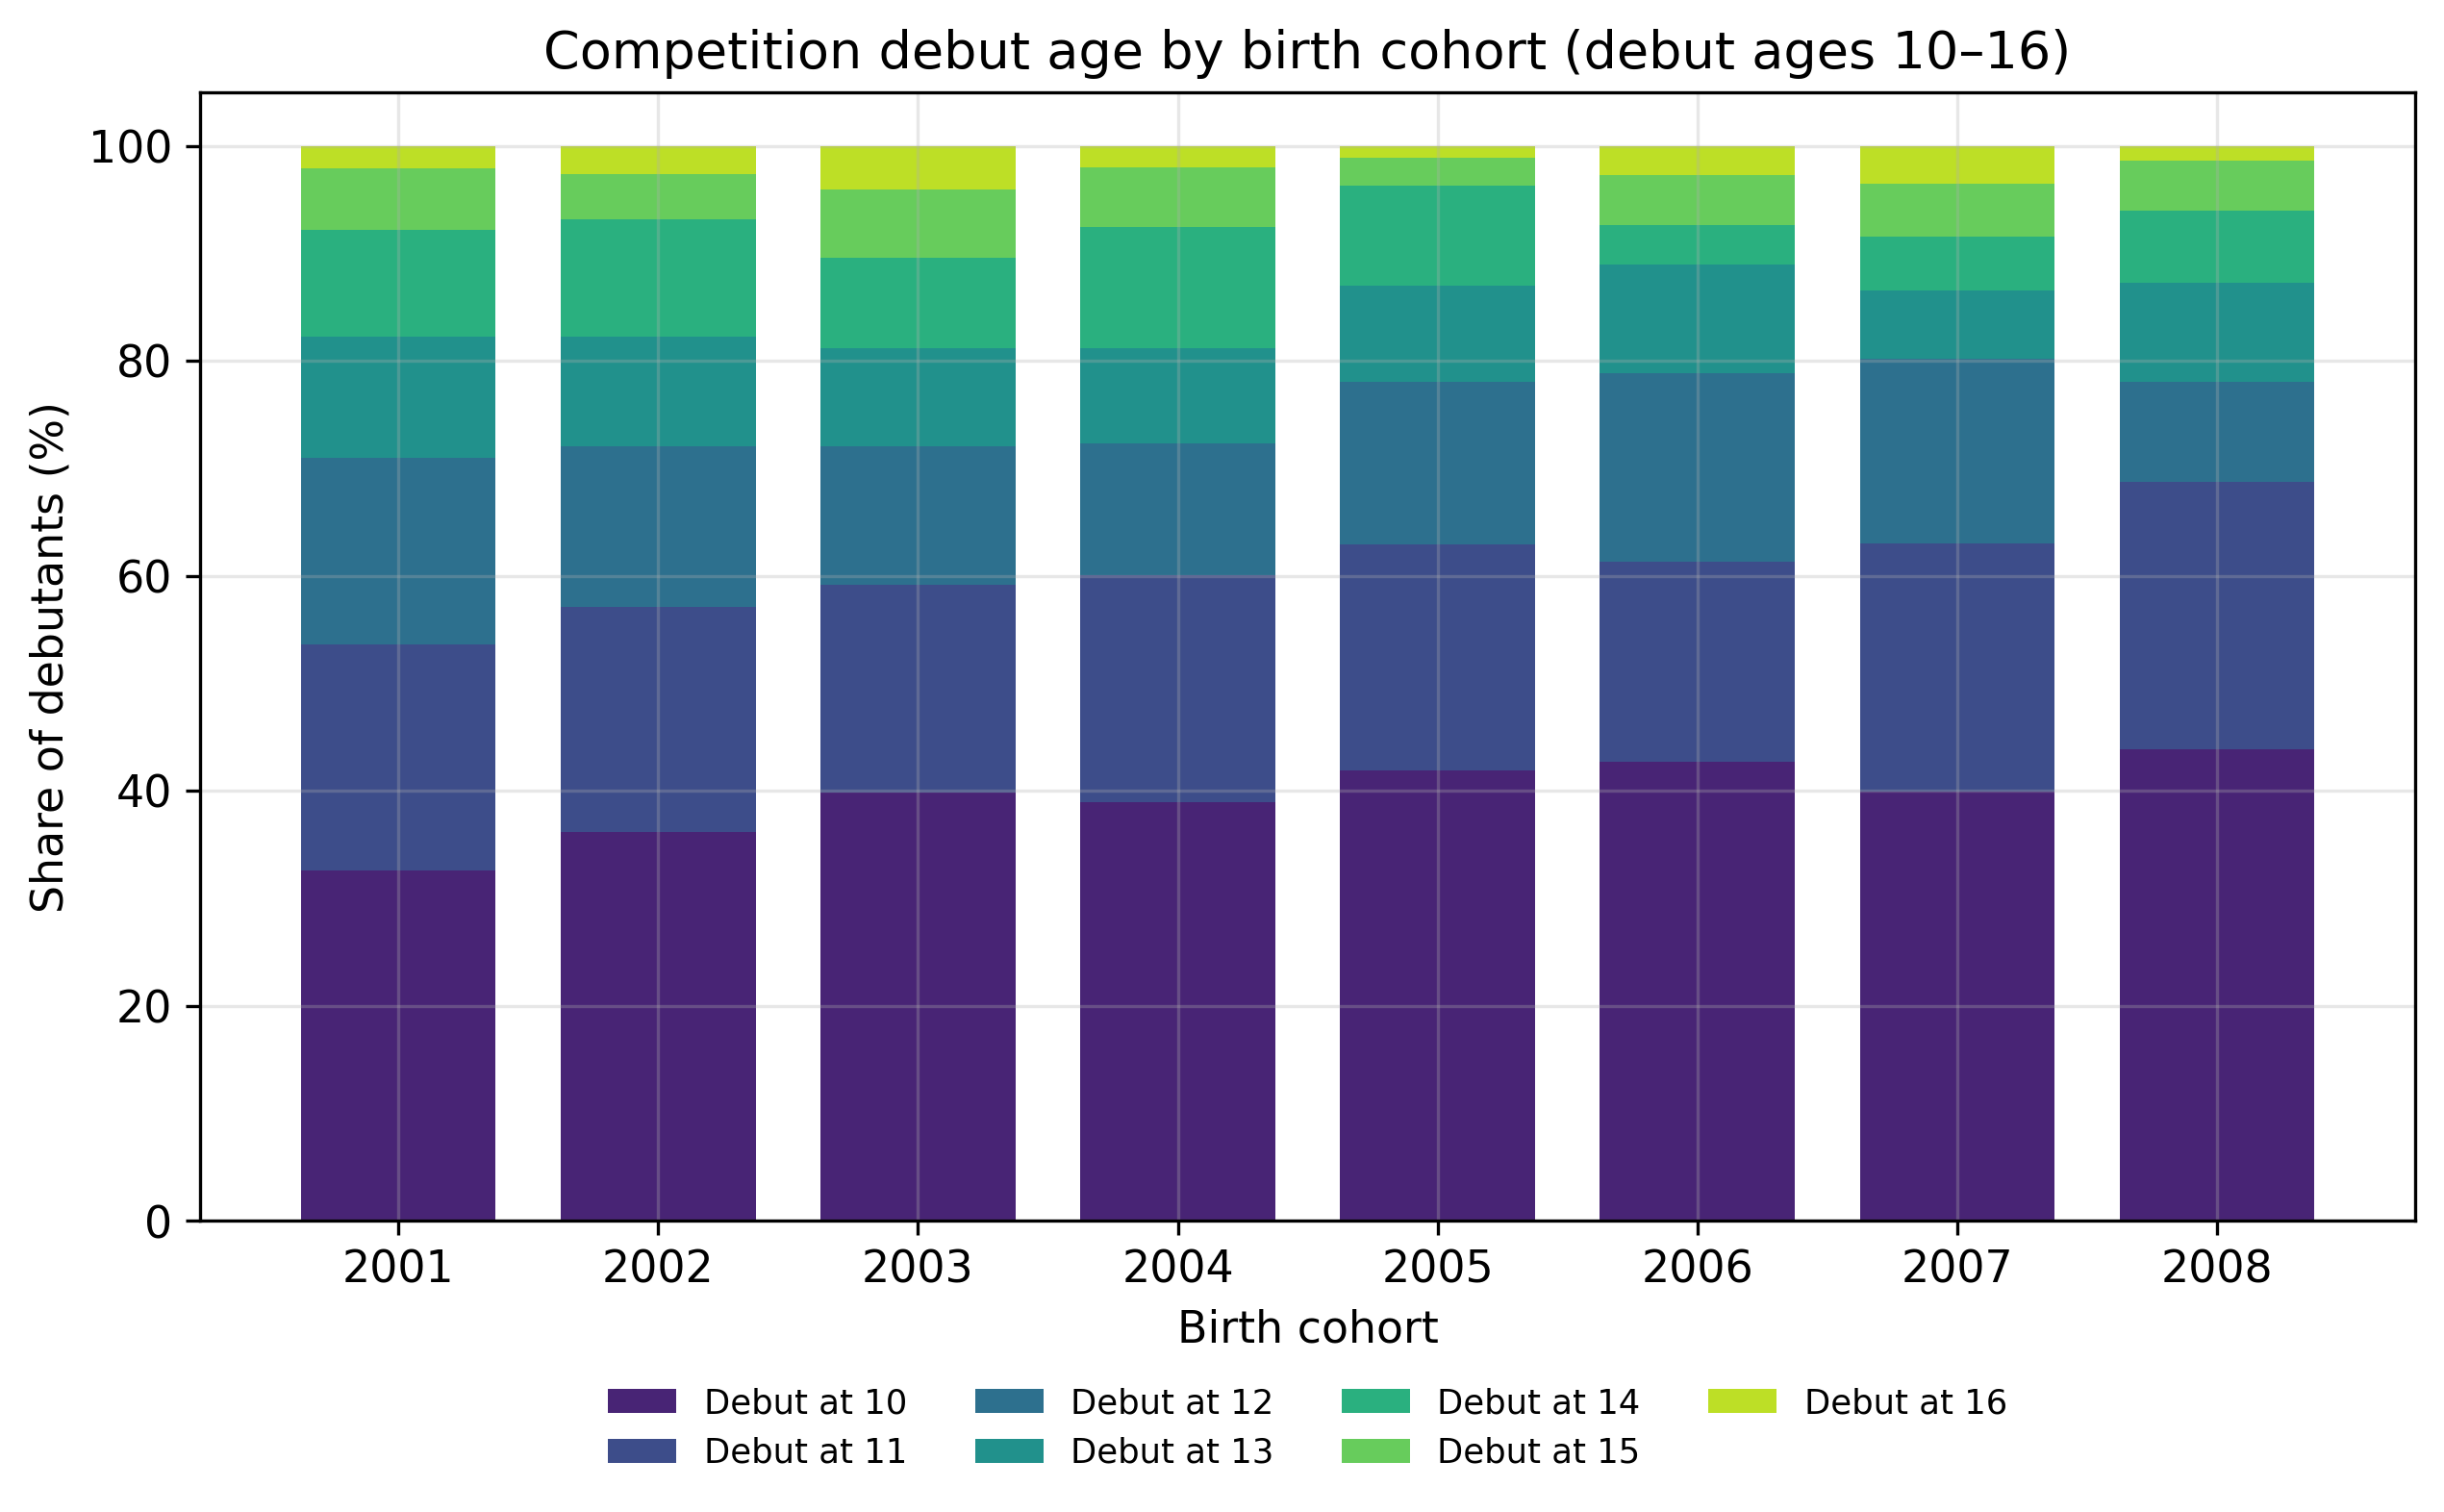
\includegraphics[width=0.85\textwidth]{fig1_debut_age_by_cohort.png}
\caption*{\textbf{Figure S1.} Competition debut age by birth cohort (all debutants born 2001--2008, debut ages 10--16).}
\end{figure}

\begin{figure}[H]
\centering
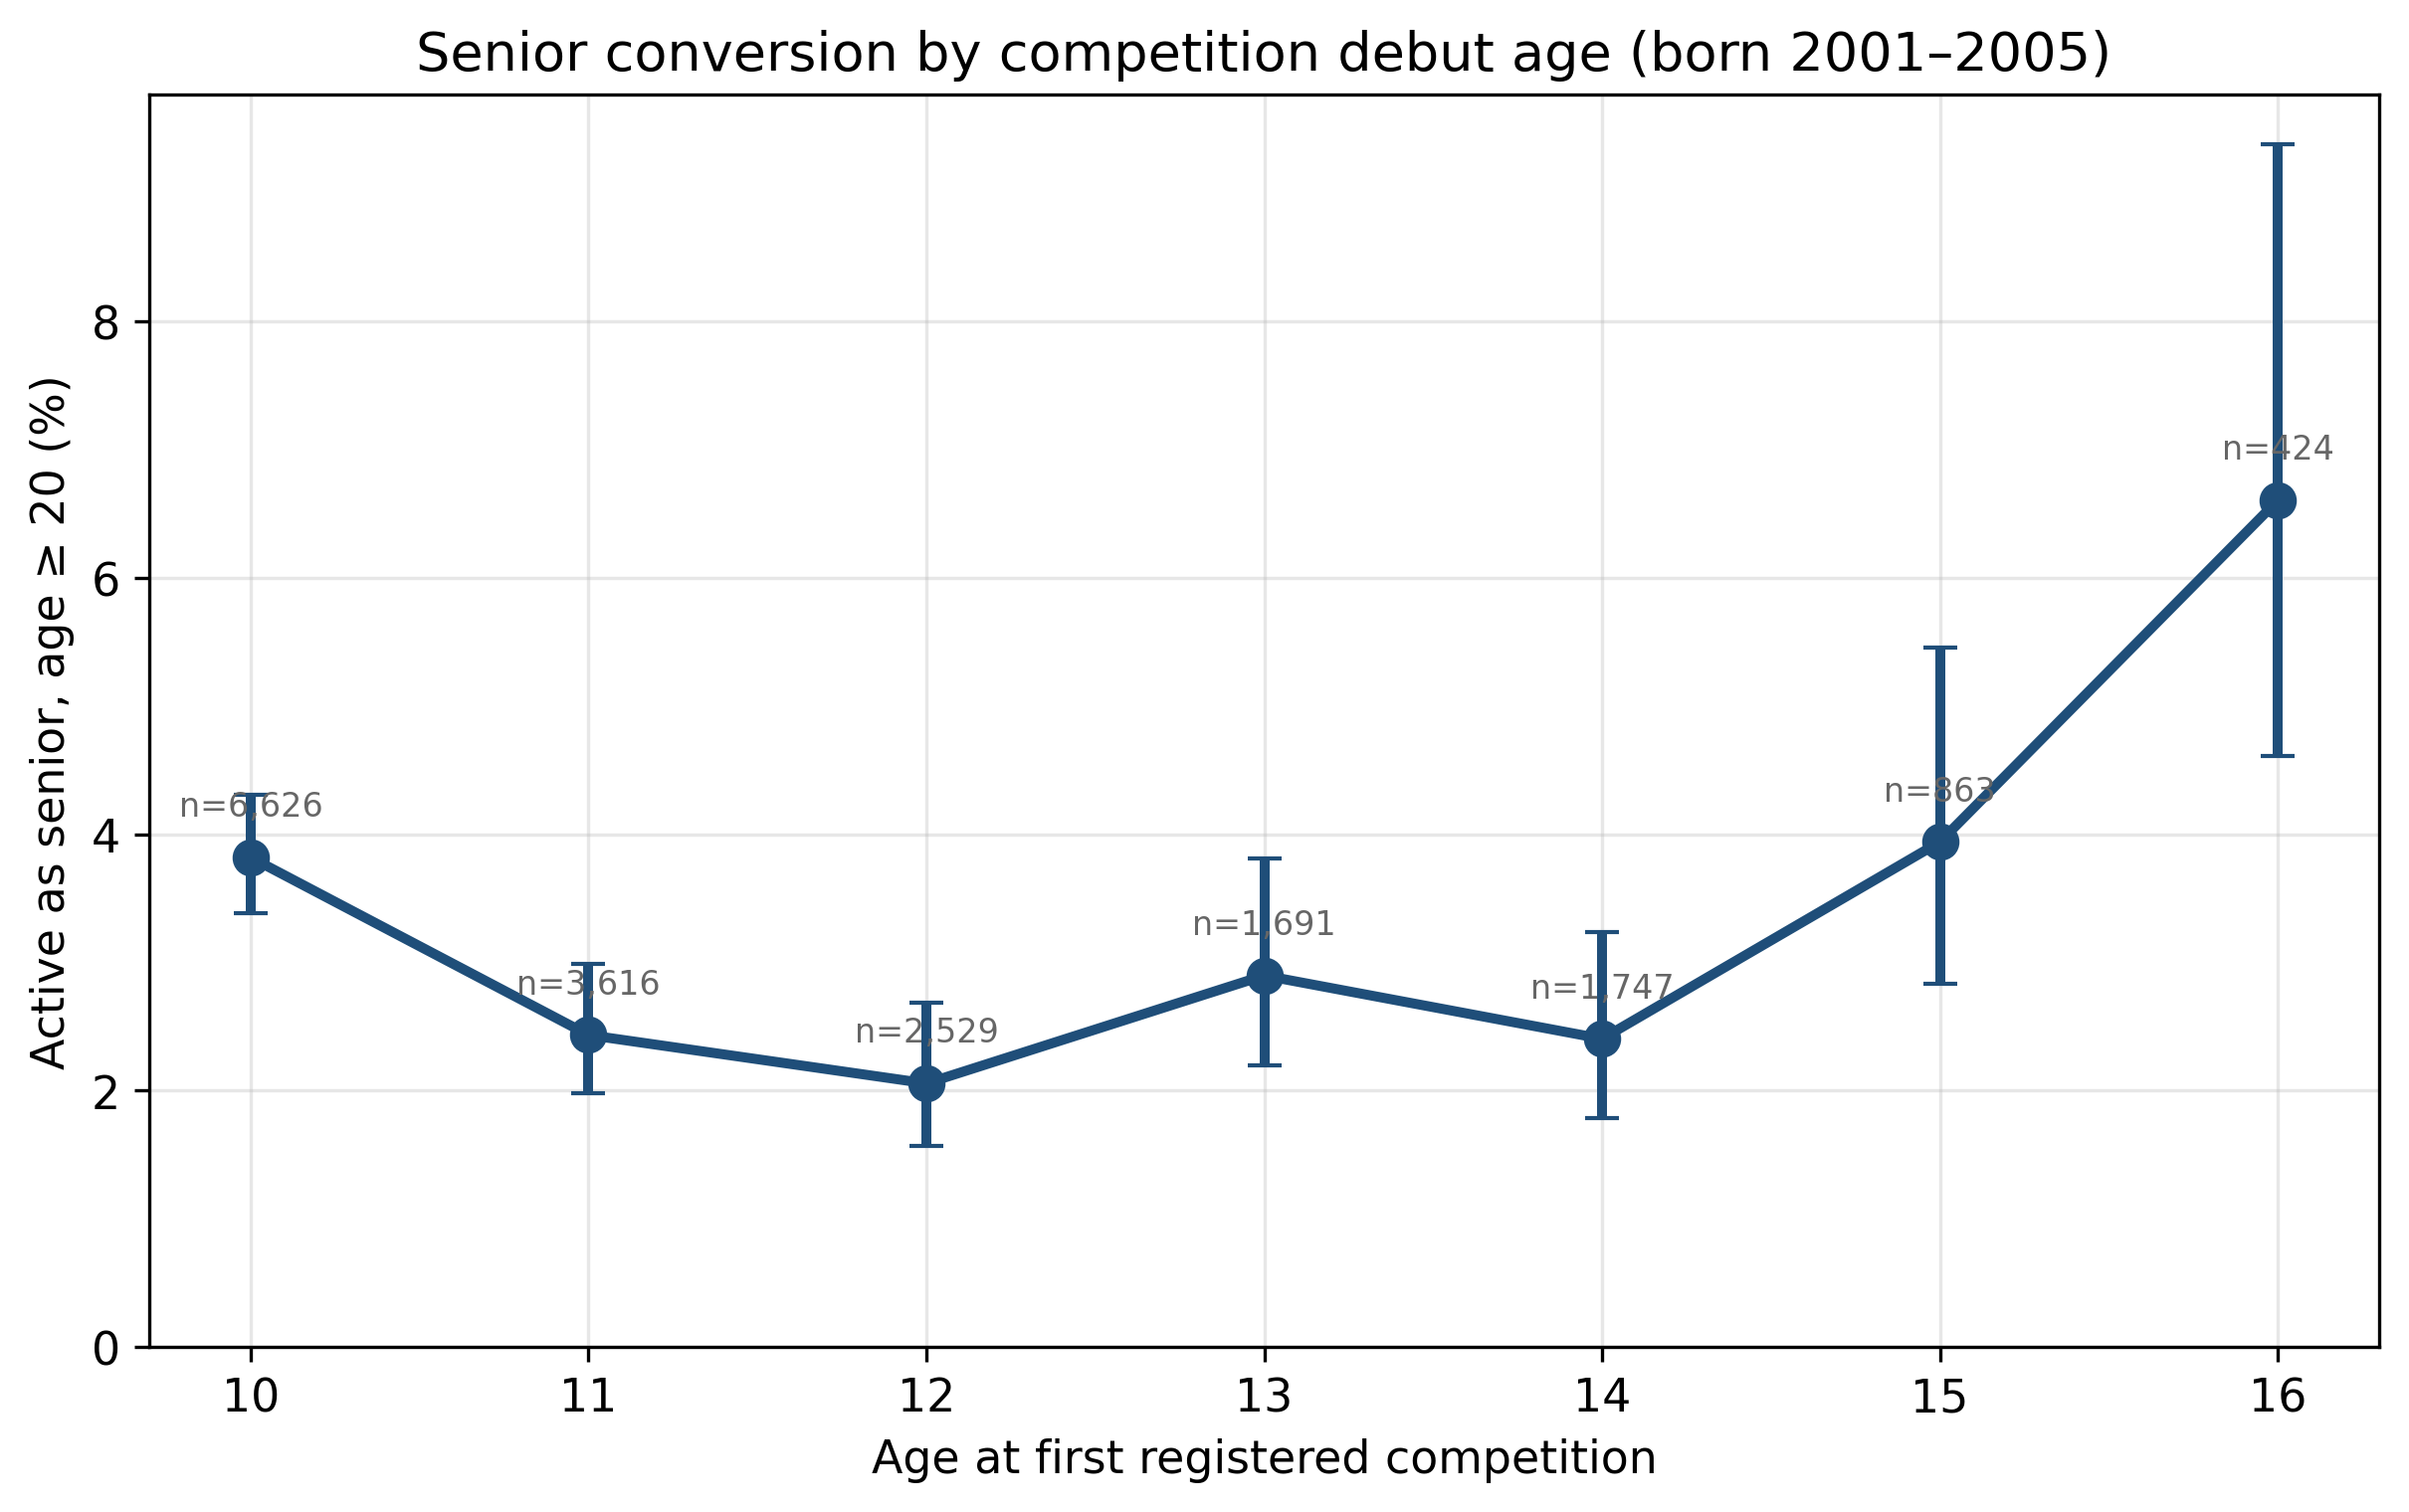
\includegraphics[width=0.85\textwidth]{fig2_senior_by_debut_age.png}
\caption*{\textbf{Figure S2.} Senior conversion by competition debut age, with Wilson 95\,\% confidence intervals (born 2001--2005).}
\end{figure}

\begin{figure}[H]
\centering
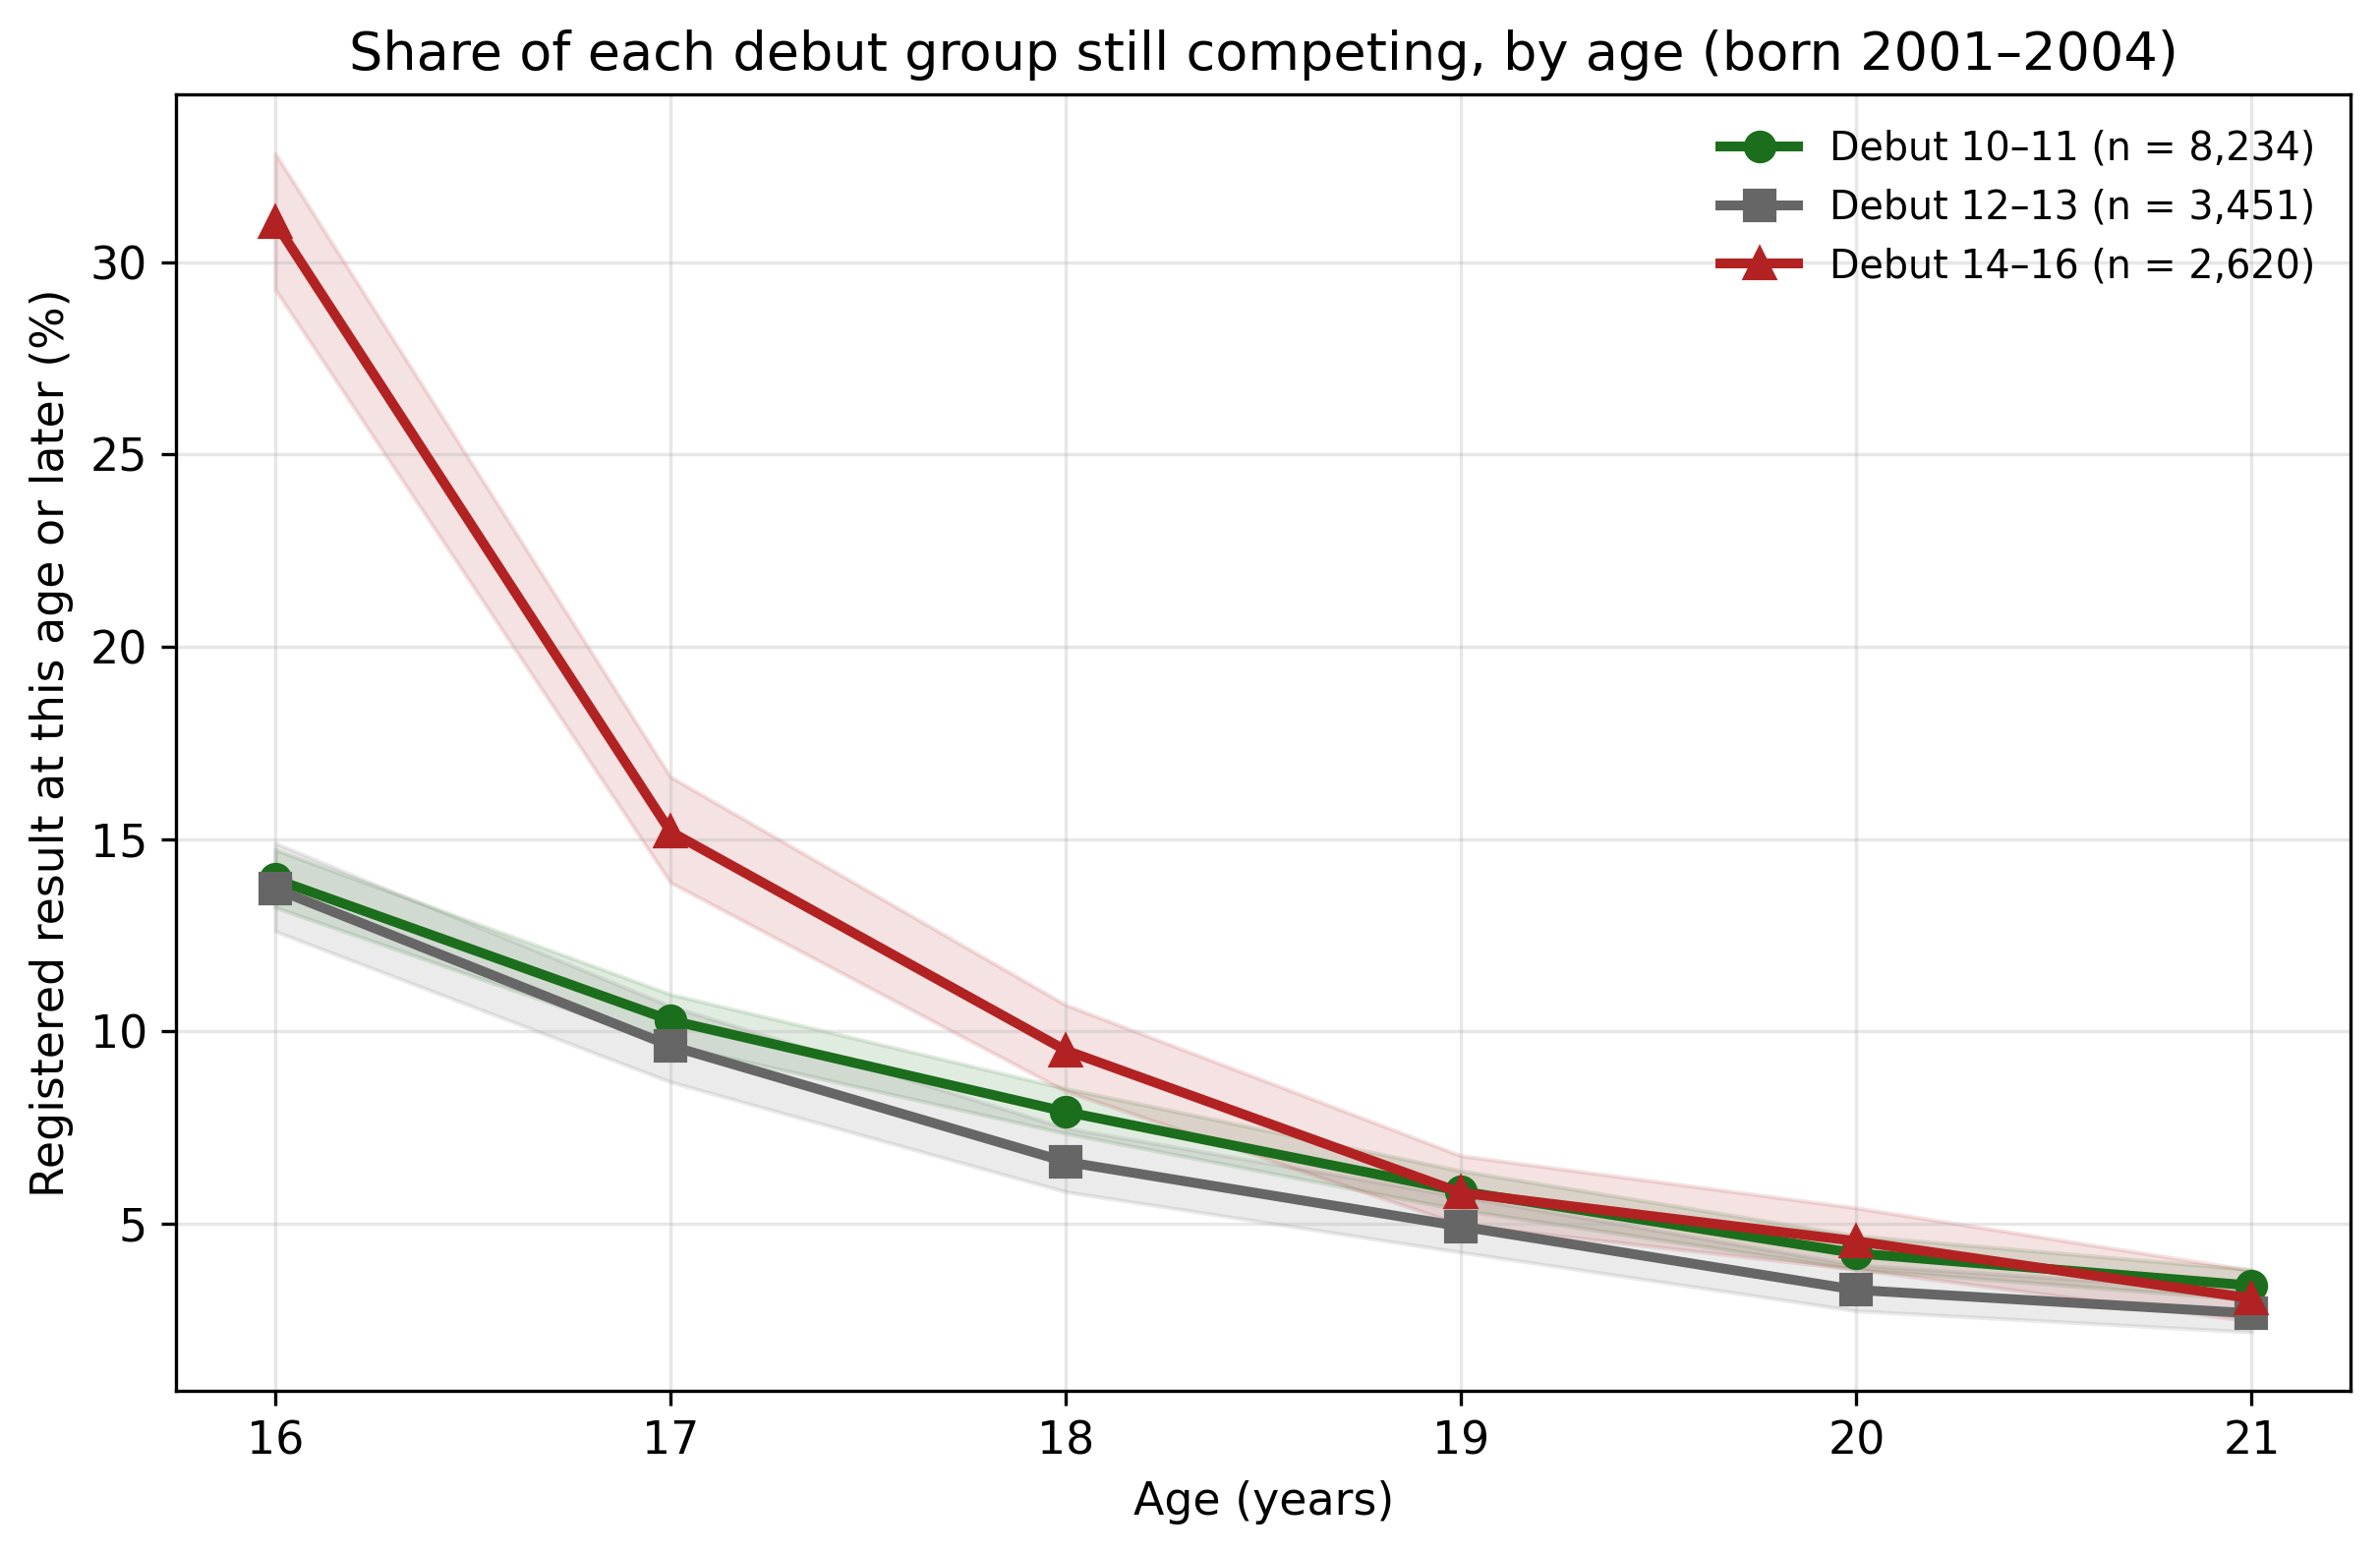
\includegraphics[width=0.85\textwidth]{fig4_shares_by_age.png}
\caption*{\textbf{Figure S3.} Share of each debut group with a registered result at that age or later, cohorts born 2001--2004 (followed to age 21 for everyone), with Wilson 95\,\% confidence bands. At 16 the late group includes the athletes who debuted at that age.}
\end{figure}

\end{document}
